\scanpage{67}
\[
\Theta=(2-\alpha_1)\rho
\]
\deleted{
\[
\sigma\sigma'-\beta=(\underbrace{2-\alpha_1}_{(4-\beta_1)=L_2(\beta_1)=})\rho
\]
\(n=3\qquad\alpha_0,\alpha_1,\alpha_2\) paramètres
\[
\boxed{\sigma\sigma'-\beta=
\underbrace{L_{n-1}(\beta_1,\mathbin{-},\beta_{n-2})}_{\unsure{\zeta_1''|\zeta_1}=L_{n-1}(}
\rho\ \unsure{?}}
\]
\[
i:n-1
\]
\[
\Psi'\Psi=\beta\operatorname{id}+\gamma\widetilde o'\otimes\widetilde o
\qquad
\left\{\begin{aligned}
\beta&=\beta_0\beta_1\mathbin{-}\beta_{n-1}\\
\gamma&=L_{n-1}(\beta_1,\mathbin{-},\beta_{n-2})
\end{aligned}\right.
\quad ?
\]
}
\figure{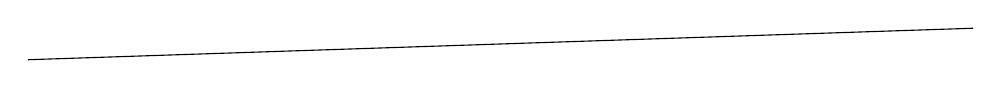
\begin{tikzpicture}\draw (0,0)--(12,0.4);\end{tikzpicture}}
\deleted{\(\unsure{\Theta}\)}
\[
\Theta(a'_{n+1})=\sigma\Psi'(a'_{n+1})+\gamma
\]
\[
\langle\underbrace{\Theta(\overbrace{a'_{n+1}}^{s'_{n+1}})}_{t_{n+1}},\Pi'\rangle
=\langle\Theta(\Pi'),\underset{a'_{n+1}}{\underbrace{s'_{n+1}}}\rangle
=-\beta\langle\Pi,s'_{n+1}\rangle=-\beta
\]
\[
u_0=s_0+s_1=2a_{-1}+a_0
\qquad\deleted{f(u)=}\langle u,\Pi\rangle=2
\]
\[
v=t_n+t_{n+1}=2t_{n+1}-\sigma a_n
\qquad\langle v,\Pi\rangle=-2\beta
\]
\[
\left\{\begin{aligned}
f(u)&=\deleted{f(s_0)+f}
4\underbrace{f(a_{-1})}_0+\underbrace{f(a_0)}_1+
2\underbrace{\varphi(a_{-1},a_0)}_{-1}=-1\\
f(v)&=\underbrace{4f(t_{n+1})}_{2\beta\sigma\gamma}
+\sigma^2\underbrace{f(a_n)}_\beta
-2\sigma\underbrace{\varphi(a_n,t_{n+1})}_{\beta\sigma}
=\beta\sigma(2\gamma-\sigma)\\
f(s_0)&=0\\
f(t_{n+1})&=\beta\widetilde\gamma\widetilde\sigma
\end{aligned}\right.
\quad\text{pour mémoire}
\]
\mspage{66}

